\chapter{Practice: Sunset Sensor}\label{sunsetSensor}
\section*{Suggested read: Chaper~\ref{ATSensorNetwork}}

In this lab assignment you will create a sunset detector using a light-dependant resistor (LDR).
If there is plenty of light, it means than the Sun is high in the sky.
During the day, the detector will light up a white LED.

In the case of complete darkness, the Sun has already gone.
At night, the detector will light up a blue LED.

The sunset detector will display an alarm (either a red LED or buzzer) for intermediate lighting ranges.

The detector consists of two parts that communicate wirelessly, namely the sensor board and the processing board.
The sensor board contains the LDR and an XBee that takes measures and sends them to the other part.
The processing board contains an XBee to receive the data and an Arduino to process it.
The processing board also contains the alarm (LED, buzzer or both).

Use a resistor in series with the LDR to obtain a range of values readable for the XBee analog input.
Take a sample every 255 ms.

On the processing board, use the API firmware to be able to serially read the values that the remote XBee is sending.
Check which is the received value and if it is in the range of interest (intermediate) activate the alarm (LED or buzzer).

\section{What you need}

\begin{itemize}
\item Breadboard (two better than one).
\item Jumper wire.
\item Arduino UNO (and USB-A-to-B cable)
\item 2 XBee S2.
\item 2 XBee explorer (and at least one USB-to-mini-USB cable)
\item Three LEDs (white, red, blue)
\item A buzzer (optional)
\item A photoresistor (or Light Dependant Resistance). ~10Kohm in the dark, ~1Kohm in bright light.
\item 20Kohm resistor.
\end{itemize}

\begin{figure}[htbp]
  \centering
  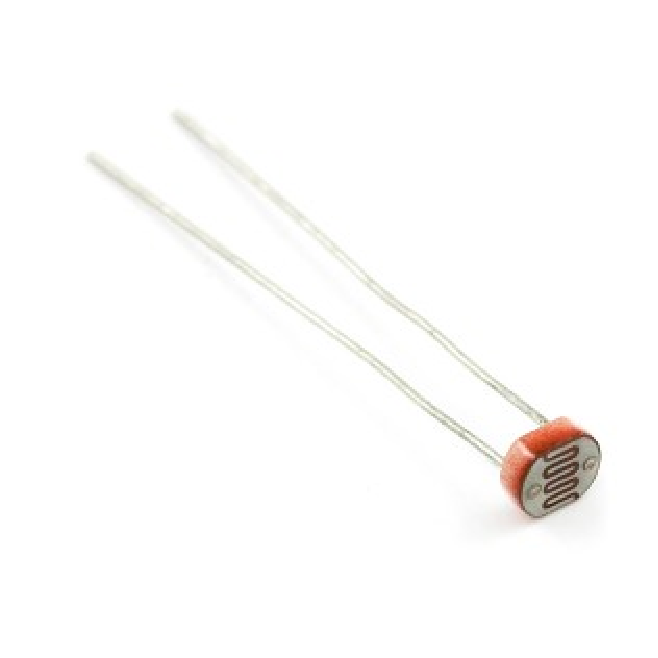
\includegraphics[width=0.3\linewidth]{figures/ldr.eps}
  \caption{LDR}
  \label{fig:ldr}
\end{figure}

\section{Configuration}
Use X-CTU to configure your XBees.
One of them must be configured as a router (e.g., router AT 22A7 at the time of writing) and the other as a coordinator API (e.g., coordinator API 21A7 at the time of writing).

For the router, configure the PANID, the destination address (both high and low), enable channel verification (Networking $\rightarrow$  JV), set D0 to analog (I/O settings $\rightarrow$  D0 $\rightarrow$  ADC) and set the sampling rate to 128 ms (I/O settings $\rightarrow$  I/O sampling $\rightarrow$  IR - I/O sampling rate $\rightarrow$  FF).

For the coordinator, you just have to configure the PANID and the destination's address.

\section{Connections}

For prototyping purposes, we will place the sensing and the processing board next to the other as in Fig. \ref{fig:sunset_sensor}, to make it possible to power both of them using the Arduino.
For real deployment, you could use batteries to power the sensor board.

Connect digital outputs 10, 11 and 12 to the LEDs.
Optionally you can also connect a buzzer if you are feeling noisy.

Connect also the LDR in series with a resistor that is twice as much the LDR (20 Kohm).
The input to the XBee is precisely the connection between the LDR and the resistor.

Make sure that the RSSI LEDs of the explorer are on, which means that both of them are in the same network.
Note that we are using the series communication pins to pass information from the XBee to the Arduino.
This wires need to be removed to program the Arduino, as the programming process also uses the serial communication port.

\begin{figure}[htbp]
  \centering
  
\includegraphics[width=0.9\linewidth]{figures/sunset_sensor.eps}
  \caption{Sunset sensor connections}
  \label{fig:sunset_sensor}
\end{figure}

\section{The code}

The following code reads a word value (2 bytes) from the serial port and blinks one of the LEDs accordingly.
The ranges of day, sunset and night might need to be adjusted. 

There is a debug LED that you can use to troubleshoot.
This LED blinks when Arduino reads data from the XBee.


\begin{lstlisting} [caption = {Sunset sensor}, language = C, label = {code:sunset_sensor}, numbers = left, escapeinside={@}{@}]
// This code is derived from Robert Faludi's book
// "Building Wireless Sensor Networks"
// Check the original for further explanations

int LED_NIGHT = 10;
int LED_SUNSET = 11;
int LED_DAY = 12;
int debugLED = 13;
int analogValue = 0;

void setup() {
    pinMode(LED_DAY,OUTPUT);
    pinMode(LED_SUNSET,OUTPUT);
    pinMode(LED_NIGHT,OUTPUT);
    pinMode(debugLED,OUTPUT);
    Serial.begin(9600);
}

void loop() {
    digitalWrite(LED_NIGHT, LOW);
    digitalWrite(LED_SUNSET, LOW);
    digitalWrite(LED_DAY, LOW);
    // make sure everything we need is in the buffer
    if (Serial.available() >= 21) {
        // look for the start byte
        if (Serial.read() == 0x7E) {
            //blink debug LED to indicate when data is received
            digitalWrite(debugLED, HIGH);
            delay(10);
            digitalWrite(debugLED, LOW);
            // read the variables that we're not using out of the buffer
            for (int i = 0; i<18; i++) {
                byte discard = Serial.read();
            }
            int analogHigh = Serial.read();
            int analogLow = Serial.read();
            analogValue = analogLow + (analogHigh * 256);
        }
    }

    if (analogValue > 0 && analogValue <= 350) {
        digitalWrite(LED_NIGHT, HIGH);
        delay(10);
        digitalWrite(LED_NIGHT, LOW);
    }

    if (analogValue > 350 && analogValue <= 750) {
        digitalWrite(LED_SUNSET, HIGH);
        delay(10);
        digitalWrite(LED_SUNSET, LOW);
    }

    if (analogValue > 750 && analogValue <= 1023) {
        digitalWrite(LED_DAY, HIGH);
        delay(10);
        digitalWrite(LED_DAY, LOW);
      }
}
\end{lstlisting}


\section{Advanced optional assignment}

If you are willing to do more complicated stuff, try to move the alarm to the sensor board. 
Now the sensor board receives the data, sends it to the processing board for processing, and waits for an instruction from the processing board to ring or light the alarm.
